\chapter{Theorie}
\label{ch:theo}

\section{MCTDH}

 Die Effizienz des MCTDH-Verfahrens resultiert aus der doppellagigen Struktur der verwendeten Wellenfunktion. In anderen Wellenpaktdynamikverfahren, 
wie der Standardmethode \cite{MCTDHreview3}, wird die Wellenfunktion direkt in einer zeitunabh"angigen Basis oder einem zeitunabh"angigen Gitter dargestellt. 
Anstatt die Wellenfunktion in einer zeitunabh"angigen Basis zu entwickeln,
erfolgt im MCTDH-Verfahren die Darstellung des korrelierten mehrdimensionalen Wellenpaketes in einem Satz zeitabh"angiger Basisfunktionen.
%wird im MCTDH-Verfahren das korrelierte mehrdimensionale Wellenpaket als ein Satz von zeitabh"angigen Basisfunktionen dargestellt.
Diese zeitabh"angigen Basisfunktionen werden Einteilchenfunktionen (von englisch \textit{single-parti\-cle function}, SPF) genannt. 
Die SPFs werden in der primitiven zeitunabh"angigen Basis oder dem Gitter ausgedr"uckt.
Das MCTDH-Verfahren kann als eine Zweilagendarstellung angesehen werden:
So bilden die Entwicklungskoeffizienten, die genutzt werden, um die korrelierte Wellenfunktion in dem Satz der SPF-Basis auszudr"ucken, die obere Lage.
Die zeitabh"angigen Entwicklungskoeffizienten, welche die zeitabh"angigen SPFs in der primitiven zeitunabh"angigen Basis darstellen, bilden die untere Lage.
Die Bewegungsgleichungen, durch die gleichzeitig die optimalen Entwicklungskoeffizienten f"ur beide Lagen bestimmt werden, ergeben sich aus dem Dirac-Frenkel Variationsprinzip.
   
Dennoch ist auch das MCTDH-Verfahren durch die Anzahl der korrelierten Koordinaten limitiert. 
Die Effizienz des MCTDH-Verfahrens resultiert aus der Gr"o"se der SPF-Basis, welche, verglichen mit der primitiven Basis, signifikant kleiner gew"ahlt werden kann.
Aller\-dings skaliert der numerische Aufwand des MCTDH-Verfahrens noch immer exponentiell mit der Anzahl der kor\-relierten Koordinaten.
Um Korrelationseffekte beschreiben zu k"onnen, sind mindestens zwei SPFs in jeder dieser Koordinaten notwendig.
Die Anzahl der Konfigurationen, die in der MCTDH-Wellenfunktion enthalten ist, betr"agt bei $ f $ kor\-relierten Koordinaten mindestens $ 2^f $ Konfigurationen.
Aufgrund dieser Limitierung konnten mit dem MCTDH-Verfahren Systeme mit maximal 12-14 kor\-relierten Koordinaten  berechnet werden.\cite{HM1, HM2, HM4, WWM, WWM2, HM5,
 WMC, BWHHM}
 
 Im von Meyer eingef"uhrten Moden-Kombinationsverfahren kann die Anzahl der Konfigurationen reduziert werden.
%Das Moden-Kombinationsverfahren wurde von Meyer und seinen Mitarbeitern eingef"uhrt \cite{EMC, WMC2}, das die Anzahl der Konfigurationen reduziert.
In diesem Verfah\-ren werden die ,,logischen`` Koordina\-ten, die in der MCTDH-Darstellung verwendet werden, von physikalischen Koordina\-ten unterschieden. 
Es werden verschiedene physikalische Koordinaten zu einzelnen logi\-schen Koordinaten kombiniert.
Analog zur Theorie der Elektronenstruktur werden diese mehrdimensionalen logischen Koordinaten Partikel genannt. 
Folglich wird die MCTDH-Rechnung statt durch die korrelierten Koordinaten durch die Partikel limitiert. 
So konn\-ten Systeme  mit 15-24 korrelierten Freiheitsgraden \cite{H5O2+MCTDH2, H5O2+MCTDH3, RWMC, CWMC}
und System-Bad-Mo\-del\-le \cite{W, WTM, NM2} durch das Moden-Kombinationsverfahren behandelt werden.
Zwar konnte durch dieses Verfahren die Grenze zu h"oherer Dimensionalit"at verschoben werden,
 dennoch bleibt die grundlegende Einschr"ankung: Der numerische Aufwand skaliert mindestens mit $2^p$, wobei $ p $ die Anzahl der logischen Koordinaten bzw.
 Partikel wiedergibt. Die Anzahl an physikalischen Koordinaten, die zu logische Koordinaten zusammengefasst werden k"onnen, ist begrenzt, da die SPFs
 nun mehrdimensionale Wellenfunktionen darstellen. F"ur molekulare Systeme stellte sich heraus, dass die Kombination von mehr als drei bis vier Koordinaten in einem Partikel
ineffizient ist.

Die Begrenzung durch die Anzahl der korrelierten Koordinaten bzw. Partikel konnte durch das Multilayer-MCTDH-Verfahren \cite{WT3} "uberwunden werden.
Die SPFs des MCTDH-Verfahrens k"onnen ebenfalls als MCTDH-Wellenfunktion dargestellt werden.
So kann z.B. eine MCTDH-Wellenfunktion um eine Lage erweitert werden, sodass die Wellenfunktion in drei Lagen ausgedr"uckt wird:
Die oberste Lage wird durch die zeitabh"angigen Entwicklungskoeffizienten gebildet. Die Wellenfunktion wird in der SPF-Basis der ersten Lage dargestellt, d.h.
den SPFs des einfachen MCTDHs. Die mittlere Lage wird durch die zeitabh"angigen Entwicklungskoeffizienten gebildet, welche die SPFs der ersten Lage in der
SPF-Basis der zweiten Lage darstellen.
D.h. die SPFs der ersten Lage werden in der SPF-Basis einer zus"atzlichen Lage ausgedr"uckt, die im Multilayer-MCTDH-Verfahren hinzugekommen ist. 
Schlie"slich werden in der untersten Lage die SPFs der zweiten Lage in der primitiven zeitunabh"angigen Basis dargestellt.
Durch eine rekursive Anwendung des MCTDH-Verfahrens k"onnen weitere Lagen hinzugef"ugt werden.
Mit dem Multilayer-MCTDH-Verfahren waren quantumdynamische Rechnungen von System-Bad Modellen mit bis zu 1000 korrelierten Koordinaten m"oglich,
in denen Elektronentransferprozesse \cite{WT3, WST} untersucht wurden.

Die Propagation der MCTDH-Wellenfunktion setzt die effiziente Berechnung der Matrixelemente des Hamiltonoperators voraus.
Solange der Hamiltonoperator der Summe von Produkten von Einteilchenoperatoren \cite{MMC1} entspricht, stellt die Berechnung der Matrixelemente kein Problem dar.
Im Gegensatz zu vielen Modelhamiltonoperatoren k"onnen \textit{ab initio} Potentialenergiefl"achen aber nur selten in dieser Form dargestellt werden.
Durch die Verwendung einer spezifischen zeitabh"angigen Quadratur, welche die Matrixelemente allgemeiner Potentiale effizient auswertet, k"onnen
auch Matrixelemente resultierend aus \textit{ab initio} Potentialenergiefl"achen effizient berechnet werden.
Dieses Verfahren wird correlation discrete variable representation (CDVR) \cite{M3, vHM2} genannt.

\section{Ansatz der Multilayer-MCTDH-Wellenfunktion}
Zun"achst  werden die Ans"atze der Wellenfunktionen der Standardmethode, des Zweilagen-MCTDHs und des moden\-kombi\-nierten MCTDH betrachtet,
 um anschlie"send den Ansatz der Multi\-layer-MCTDH-Wellenfunktion
stufenweise vorzustellen.

In der Standardmethode wird die Wellenfunktion in einer zeitunabh"angigen Basis bzw. in einem zeitunabh"angigen Gitter dargestellt.
Die mehrdimensionale Wellenfunktion wird durch das direkte Produkt von eindimensionalen Basisfunktionen $\mathcal{X}^{\kappa}_{j}(x_{\kappa})$ wie folgt 
dargestellt:

 \begin{equation}
 \Psi(x_{1},..., x_{f}, t)=\sum^{N_{1}}_{j_{1}=1} ... \sum^{N_{f}}_{j_{f}=1} A^{1}_{j_{1}, ..., j_{f}}(t)\cdot \mathcal{X}^{(1)}_{j_{1}}(x_{1}) \cdot ... \cdot \mathcal{X}^{(f)}_{j_{f}}(x_{f})
 \label{Eq:Std_wave}
 \end{equation}

Die zeitabh"angigen Koeffizienten $A^{1}_{j_{1}, ..., j_{f}}(t)$ beschreiben die Bewegung der Wellenpakete.
Die Darstellung der Wellenfunktion in Gleichung  \ref{Eq:Std_wave} kann auch als einlagige Darstellung angesehen werden
und die Hochzahl 1 von $A^{1}_{j_{1}, ..., j_{f}}(t)$ soll darauf hinweisen, dass $A^{1}_{j_{1}, ..., j_{f}}(t)$ ein Entwicklungskoeffizient
der ersten (und einzigen) Lage ist.
\\Im MCTDH-Verfahren wird eine zus"atzliche Lage f"ur die Darstellung der Wellenfunktion eingef"uhrt.
Die mehrdimensionale Wellenfunktion wird erst in einer orthonormalen Basis der zeitabh"angigen SPFs $\phi^{1;\kappa}_{j}(x_{\kappa},t)$
entwickelt.


 \begin{equation}
 \Psi(x_{1},..., x_{f}, t)=\sum^{n_{1}}_{j_{1}=1} ... \sum^{n_{f}}_{j_{f}=1} A^{1}_{j_{1}, ..., j_{f}}(t)
 \cdot \phi^{1;1}_{j_{1}}(x_{1}, t) \cdot ... \cdot \phi^{1;f}_{j_{f}}(x_{f}, t).
 \label{Eq:mctdh_wave}
 \end{equation}

Anschlie"send werden diese SPFs innerhalb der zeitunabh"angigen primitive Basis darge\-stellt: 

\begin{equation}
 \phi^{1;\kappa}_{m} (x_{\kappa}, t)=\sum^{N_{\kappa}}_{j=1} A^{2;\kappa}_{m;j}(t) \cdot \mathcal{X}^{(\kappa)}_{j}(x_{\kappa}).
 \label{Eq:SPF}
 \end{equation}

Gleichung \ref{Eq:SPF} beinhaltet einen Satz zus"atzlicher Entwicklungskoeffizienten, $ A^{2;\kappa}_{m;j}(t) $, der die zeitabh"angigen SPFs
in der zeitunabh"anigen primitiven Basis darstellt.
Die hochgestellte Zahl $z$ der Koeffizienten $A^{z}(t)$ bezieht sich auf die Lagentiefen.
In Glei\-chung \ref{Eq:SPF} folgt aus $z=2$, dass Gleichung \ref{Eq:SPF} die zweite Lage darstellt.
Das hochgestellte $\kappa$ und der Index $m$ von $A^{2;\kappa}_{m;j}(t)$ beziehen sich auf die $m$-te SPF der $\kappa$-ten Koordinate.

%Zur Visualisierung der Lagenstruktur des MCTDHs dienen die Diagramme f"ur die unterschiedlichen Darstellungen der Wellenfunktionen in Abbildung \ref{fig:tree}.
Zur Visualisierung unterschiedlicher MCTDH-Wellenfunktionen, f"ur die unterschiedlich viele Lagen verwendet wurden, dienen Baumdiagramme \cite{Mreview2},
wie sie in Abbildung \ref{fig:tree} gezeigt werden.
Als Beispiel soll ein siebendimensionales System dienen.
Die Standardwellenpaketdarstellung aus Glei\-chung \ref{Eq:Std_wave} und die MCTDH-Darstellung sind in Abbildung \ref{fig:a} und \ref{fig:b} schematisch dargestellt.
In den Diagrammen sind die verschiedenen S"atze der A-Koeffizienten durch die ausgef"ullten schwarzen Kreise gekennzei\-chnet.
So kommt in Abbildung \ref{fig:a} ein Satz von Koeffizienten $A^{1}_{j_{1}, ..., j_{7}}$ vor, der durch den
einzigen schwarzen Punkt gekennzei\-chnet ist. 
Jede Linie, die von solchen Kreisen f"uhrt, entspricht einem tiefgestellten Index aus $ A^{1}_{j_1...j_7} $ und die Zahl neben einer Linie gibt den maximalen
Wert des Indexes an, d.h. die jeweilige Basisgr"o"se. Die tieferliegende primitive Darstellung wird durch den Koordinatdeskriptor $x_n$ hervorgehoben.
Beispielsweise ist der Koeffizient $A^{2;1}_{m;j}$ in Gleichung \ref{Eq:SPF}, der die SPFs $ \phi^{1;1}_{j_1} (x_{1}, t) $ spezifiziert, in Abbildung \ref{fig:b} mit dem 
Koeffizienten $A^1$ "uber eine Linie verbunden, die den $m$-ten Index darstellt. "Uber eine weitere Linie, die f"ur den $j$-ten Index steht,
ist  $A^{2;1}_{m;j}$ mit dem Koordinatdeskriptor $x_1$ verbunden.
In Abbildung \ref{fig:a} ist der Koeffizient $A^{1}_{j_{1}, ..., j_{7}}$  durch sieben Linien mit den entsprechenden Indizes von 
$j_1$ bis $j_7$ direkt mit den sieben Koordinatdeskriptoren $x_1,x_2,...,x_7$ verbunden und in Abbildung \ref{fig:b} ist $A^{1}_{j_{1}, ..., j_{7}}$
mit den sieben S"atzen an A-Koeffizienten $A^{2;1},A^{2;2},...,A^{2;7}$ verbunden.
Die Wellenfunktion aus Abbildung \ref{fig:a} ist direkt 
in der zeitunabh"angigen primitiven Basis dargestellt. In Abbildung \ref{fig:b} gibt es eine intermedi"are Lage an zeitabh"angigen SPFs. 

W"ahrend in den Gleichungen \ref{Eq:mctdh_wave} und \ref{Eq:SPF} nur eindimensionale SPFs vorkommen, werden im modenkombinierten MCTDH-Verfahren
mehrdimensionale SPFs verwendet. 
Hier\-f"ur werden die $f$ physikalischen Koordinaten $x_{1}, x_{2}, ..., x_{f}$  $d$ logischen Gruppen zugeordnet, die Partikel genannt werden.
Die mehrdimensionalen Koordinaten $q^{1}_{1}, q^{1}_{2}, ..., q^{1}_{d}$ sind wie folgt definiert:


\begin{align*}
  q^{1}_{1} &= \{q^{2;1}_{1},q^{2;1}_{2},q^{2;1}_{d_{1}}\}\\ 
            &= \{x_{1}, x_{2}, ..., x_{d_1}\} \\
  q^{1}_{2} &= \{q^{2;2}_{1},q^{2;2}_{2},q^{2;2}_{d_{2}}\}\\ 
            &= \{x_{d_{1}+1}, x_{d_{1}+2}, ..., x_{d_{1}+d_{2}}\} \\
            &\vdots\\
  q^{1}_{f^1} &= \{q^{2;d}_{1},q^{2;d}_{2},q^{2;d}_{d_{d}}\} \\
            &= \{...,x_{f}\}
\end{align*}


Die logische mehrdimensionale Koordinate $ q^1_\kappa $ umfasst $d_\kappa $ Koordinaten:  $q^{2;\kappa}_1, q^{2;\kappa}_2, ..., q^{2;\kappa}_{d_\kappa} $.
Die Hochzahlen 1 und 2 in dieser Notation zeigen, ob die Koordinate eine mehrdimensionale Koordinate der ersten Lage ist oder einer Koordinate
der zweiten Lage entspricht. F"ur die Koordinate der zweiten Lage gibt der zus"atzliche hochgestellter Index $\kappa$
den Index der Koordinate der ersten Lage an.
Eine modenkombinierte MCTDH-Wellenfunktion mit $d$ logischen Koordinaten wird wie folgt definiert:

\begin{equation}
 \Psi(q^{1}_{1},q^{1}_{2},..., q^{1}_{d}, t)=\sum^{n_{1}}_{j_{1}=1} ... \sum^{n_{d}}_{j_{d}=1} A^{1}_{j_{1}, ..., j_{d}}(t)
 \cdot \phi^{1;1}_{j_{1}}(q^1_{1}, t) \cdot ... \cdot \phi^{1;d}_{j_{d}}(q^1_{d}, t)
 \label{Eq:mode_comb_wave}
 \end{equation}

\begin{equation}
  \begin{gathered}
 \phi^{1;\kappa}_{m} (q^1_{\kappa}, t)=\sum^{N_{\alpha}}_{j=1} ... \sum^{N_{\beta}}_{j_{d_\kappa}=1} A^{2;\kappa}_{m;j_1,...,j_{d_\kappa}}(t)
 \cdot \mathcal{X}^{(\alpha)}_{j_1}(q^{2;\kappa}_1) \cdot ... \cdot
 \mathcal{X}^{(\beta)}_{j_{d_\kappa}}(q^{2;\kappa}_{d_\kappa})\\
 \left(\text{mit } \alpha = 1 + \sum^{\kappa - 1}_{i=1}d_i \text{ und }  \beta = 1 + \sum^{\kappa}_{i=1}d_i\right)
 \label{Eq:mode_SPF}
\end{gathered}
 \end{equation}

In Abbildung \ref{fig:c} ist das entsprechende Diagramm der Wellenfunktion eines siebendimensionalen Systems dargestellt, dessen Koordinaten 
in logischen Koordinaten zusammengefasst wurden.
Die physikalischen Koordinaten bilden in Abbildung \ref{fig:c} drei mehrdimensionale logische Koordinaten:
 $q^{1}_{1} = \{x_1, x_2\}$, $ q^{1}_{2} = \{x_3, x_4\}$
und $ q^{1}_{3} = \{x_5, x_6, x_7\}$.


\begin{figure}
    \centering
    \captionsetup[subfigure]{position=top, labelfont=bf,textfont=normalfont,singlelinecheck=off,justification=raggedright,labelformat=empty}
    \begin{subfigure}{\textwidth}
        \caption{}\label{fig:a}
    \end{subfigure}
    \begin{subfigure}{\textwidth}
        \caption{}\label{fig:b}
    \end{subfigure}
    \begin{subfigure}{\textwidth}
        \caption{}\label{fig:c}
    \end{subfigure}
    \begin{subfigure}{\textwidth}
        \caption{}\label{fig:d}
    \end{subfigure}
    \begin{subfigure}{\textwidth}
        \caption{}\label{fig:e}
    \end{subfigure}
    \begin{subfigure}{\textwidth}
        \caption{}\label{fig:f}
        \vspace*{-4cm}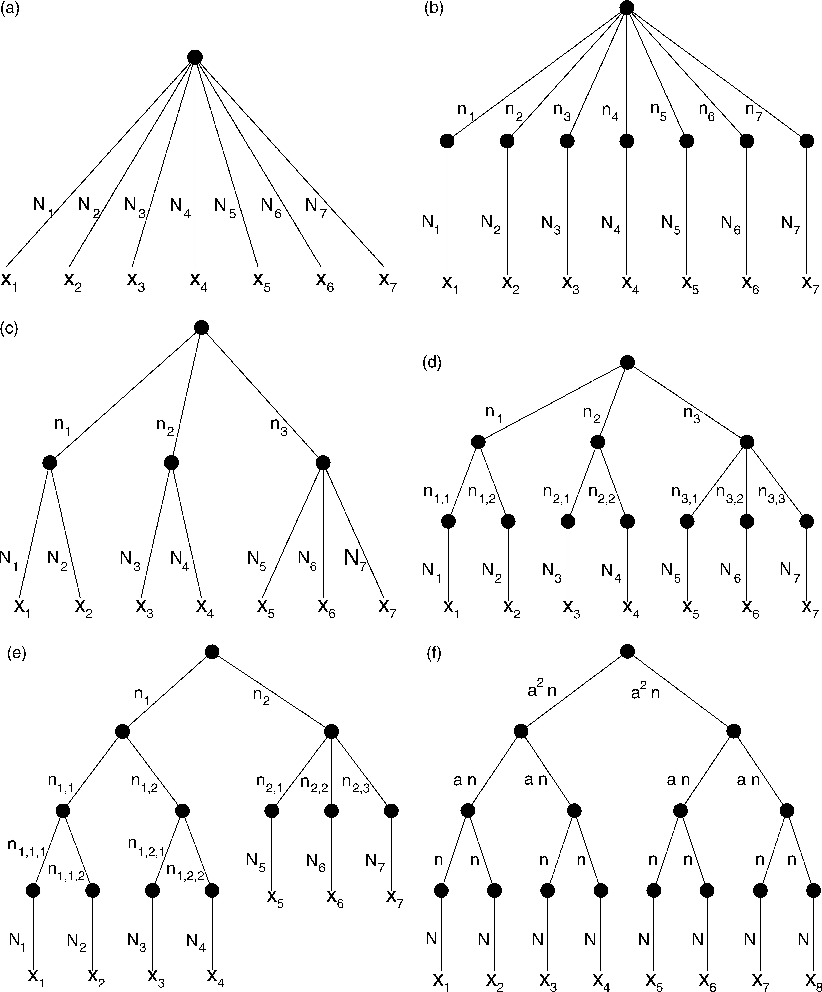
\includegraphics[width=\textwidth]{figures/treeDiagramms}
    \end{subfigure}
    \caption{Unterschiedliche Darstellungen von Wellenfunktionen eines siebendimensionalen Systems. Dargestellt sind: (a) Eine Darstellung eines Standardwellenpakets,
      (b) eine MCTDH-Wellenfunktion, (c) eine modenkombinierte MCTDH-Wellenfunktion, [(d) und (e)] eine Multilayer-MCTDH-Wellenfunktion. Die Diagramme wurden aus Ref.\cite{Mreview2} 
      entnommen.} \label{fig:tree}
\end{figure}

Im einfachsten Fall kommen im Multilayer-MCTDH zwei Lagen von SPFs vor.
Anstelle die SPFs aus Gleichung \ref{Eq:mode_comb_wave} in der primitiven zeitunabh"angigen Basis zu entwickeln,
% wie es bereits im modenkombinierte MCTDH-Verfahrens in Gleichung \ref{Eq:mode_comb_wave} durchgef"uhrt wurde,
k"onnen die mehrdimensionalen SPFs ebenfalls durch das MCTDH-Verfahren dargestellt werden.
Diese Entwicklung resultiert in einer Multilayer-MCTDH-Wellenfunktion. 
Der Ansatz der Multilayer-MCTDH-Wellenfunktion ist gegeben durch 

\begin{equation}
  \Psi(q^{1}_{1},q^{1}_{2},..., q^{1}_{d}, t)=\sum^{n_{1}}_{j_{1}=1} ... \sum^{n_{d}}_{j_{d}=1} A^{1}_{j_{1}, ..., j_{d}}(t)
  \cdot \phi^{1;1}_{j_{1}}(q^1_{1}, t) \cdot ... \cdot \phi^{1;d}_{j_{d}}(q^1_{d}, t)
  \label{Eq:ml_mctdh_wave}
  \end{equation}

\begin{align}
  \begin{split}
 \phi^{1;\kappa}_{m} (q^1_{\kappa}, t) & =  \phi^{1;\kappa}_{m} (q^{2;\kappa}_1..., q^{2;\kappa}_{d_{\kappa}},t)\\
 & = \sum^{n_{\kappa,1}}_{j=1} ... \sum^{n_{\kappa,d_\kappa}}_{j_{d_\kappa}=1} A^{2;\kappa}_{m;j_1,...,j_{d_\kappa}}(t) \\
 & \times \phi^{2;\kappa,1}_{j_1} (q^{2;\kappa}_{1}, t) \cdot ... \cdot
 \phi^{2;\kappa,d_\kappa}_{j_{d_\kappa}} (q^{2;\kappa}_{d_\kappa}, t),
\\
 \phi^{2;\kappa, \lambda}_{m} (q^{2;\kappa}_{\lambda}, t)&= \sum^{N_{\alpha}}_{j=1} A^{3;\kappa, \lambda}_{m;j}(t)
 \mathcal{X}^{(\alpha)}_{j}(q^{2;\kappa}_\lambda)
 \label{Eq:ml_mctdh_mode_SPF}
  \end{split}
 \end{align}

 \begin{equation}
  \left( \text{ mit } \alpha = \lambda + \sum^{\kappa - 1}_{i=1}d_i \right).
 \end{equation}

In Gleichung \ref{Eq:ml_mctdh_mode_SPF} ist $ \phi^{2;\kappa, \lambda}_{m}  $ 
mit der dazugeh"origen Koordinate $q^{2;\kappa}_\lambda$ eine SPF der zwei\-ten Lage.
Die Hochzahl 2 bezieht sich auf die Lagentiefe, sodass die SPF zur zweiten Lage geh"ort, 
wobei $\kappa$ und $\lambda$ die dazugeh"origen Koordinaten kennzeichnen.
Die Ent\-wicklungskoeffizienten $A^{3;\kappa, \lambda}_{m;j}(t) $ werden verwendet, um diese SPF darzustellen
und die Entwicklungskoeffizienten $A^{2;\kappa}_{m;j_1,...,j_{d_\kappa}}(t)$ definieren die Entwicklung der SPFs der ersten Lage, die
in der SPF-Basis der zweiten Lage entwickelt werden.
In Gleichung \ref{Eq:SPF} definier\-ten diese Entwicklungskoeffizienten die SPFs der ersten Lage in der primitiven zeitunabh"angigen Basis.
Abbildung \ref{fig:d} zeigt das entsprechende Diagramm f"ur ein siebendimensionales System in Multilayer-MCTDH-Darstellung.

Da die Gleichungen der Multilayer-MCTDH-Wellenfunktion schnell unhandlich werden, ist es einfacher, statt der Gleichungen die Wellenfunktionen 
wie in Abbildung \ref{fig:tree}
als Diagramm anzugeben. Jedes Diagramm definert die Wellenfunktionen eindeutig, sodass aus den Diagrammen die entsprechenden
Gleichungen der Wellenfunktionen abgelei\-tet werden k"onnen.
Die Notation f"ur die SPFs, A-Koeffizienten und (mehrdimensionalen) Koordinaten, die oben in den Gleichungen angegeben wurde,
kann einfach f"ur beliebig mehrlagige Darstellungen erweitert werden. 
Ein Beispiel dieser Strukturen ist in Abbildung \ref{fig:e} dargestellt. 
Die Anzahl der Lagen f"ur die jeweiligen Koordinaten kann bis zur primitiven Darstellung von 
Koordinate zu Koordinate variieren.
So wird in Abbildung \ref{fig:e} das Baumdiagramm einer Multilayer-MCTDH-Wellfunktion gezeigt, 
in der f"ur die Koordinaten $ x_1-x_4 $ drei MCTDH-Lagen verwendet werden 
(d.h. insgesamt eine Vier-Lagen-Darstellung)
und f"ur die Koordinaten $ x_5 - x_7 $  werden zwei MCTDH-Lagen verwendet (d.h. eine Drei-Lagen-Darstellung).

